\chapter{系统的稳定性}
\section{稳定性的基本概念}
\begin{definition}
    称系统是稳定的，当且仅当在扰动消除后，系统能够以足够的准确度恢复到原来的平衡状态，否则称系统是不稳定的
\end{definition}

\section{线性定常系统稳定的充要条件}
\begin{theorem}
    线性定常系统稳定的充要条件为：闭环系统特征方程的根全部具有负实部。或者说，闭环传递函数极点全部在S平面的左半平面
\end{theorem}

\section{Routh稳定判据}
\begin{definition}{Routh稳定判据}
    特征方程如果同时满足下面三个条件，闭环系统是稳定的：
    \begin{enumerate}
        \item 特征方程按降幂排列不存在缺项情况
        \item 特征方程的各项系数全是实数
        \item 用特征方程的各项系数排成Routh行列表，表中第一列各元全部大于零
    \end{enumerate}
\end{definition}
\begin{definition}
    Routh行列表如下：
    \begin{equation*}
        \begin{array}{cccccc}
            s^n & a_n& a_{n-2} & a_{n-4} & a_{n-6} & \cdots \\
            s^{n-1}&  a_{n-1} & a_{n-3} & a_{n-5} & a_{n-7} & \cdots \\
            s^{n-2} & b_1 & b_2 &b_3 & \cdots & \cdots \\
            \vdots  & c_1 & c_2 &c_3 & \cdots &\cdots \\
            s^2 & \vdots & \vdots & \vdots & \ddots & \\ 
            s^1 & \vdots & \vdots & \vdots & & \ddots \\
            s^0 & \vdots & \vdots & \vdots &\cdots & \cdots 
        \end{array}
    \end{equation*}
    
    其中：
    \begin{equation*}
        \begin{split}
            & b_1 = \frac{a_{n-1 }a_{n-2}-a_{n} a_{n-3}}{a_{n-1}} \\
            & b_2 = \frac{a_{n-1}a_{n-4}-a_n a_{n-5}}{a_{n-1}} \\
            & \vdots \\
            & c_1 = \frac{b_1 a_{n-3}- a_{n-1} b_2} {b_1} \\
            & c_2 = \frac{b_1 a_{n-5} - a_{n-1} b_3}{b_1}
        \end{split}
    \end{equation*}

    用文字表述如下：
    \begin{enumerate}
        \item 前两行：跳项写，缺项时写0
        \item 其他行计算（第i列）：取第i+1列与第一列做$2\times2$行列式然后除以上一行的第一项
    \end{enumerate}
    一些特殊情况的处理方法：
    \begin{enumerate}
        \item 上一行的第一项为0：将该项改为无穷小$\xi$，再做上述计算，最后取$\xi\rightarrow 0$的极限
        \item 若存在一行全零（全零行）：取全零行的上一行构造辅助方程，对该方程求导之后将对应系数填到该行中，再做上述计算
    \end{enumerate}
\end{definition}

\begin{property}
    Routh行列表具有以下性质：
    \begin{enumerate}
        \item 在计算Routh行列表时，用同一个正数去乘（或除）某一行的各元，不会影响稳定性判定结构。这样做往往能简化以后的运算
        \item Routh行列表第一列元自上而下符号改变的次数等于闭环系统特征方程中具有正实部根的个数（注：0不算改变符号！）
    \end{enumerate}
\end{property}

\begin{example}
    系统的特征方程为：
    \begin{equation*}
        D(s) = s^6 + 4s^5 - 4s^4 + 4s^3 - 7s^2 - 8s + 10 = 0
    \end{equation*}

    求该系统在右半平面特征根的数目

    \textbf{解}： 因为特征方程各项系数有正有负，所以系统不稳定。列Routh行列表：
    \begin{equation*}
        \begin{array}{cccccc}
            s^6 & 1             & -4 & -7 & 10 & \\
            s^5 & 4             & 4  & -8 & 0  & \\
            s^4 & -5            & -5 & 10 &    & \text{各元除以5}\\
                & -1            & -1 & 2  &    & \\
            s^3 & 0             & 0  &    &    & \text{做辅助方程}-s^4 -s^2 +2 = 0\\
                & -4            & -2 &    &    & \text{求导得}-4s^3 -2s = 0 \\
            s^2 & -\frac{1}{2}  & 2  &    &    & \text{各元同乘以2} \\
                & -1            & 4  &    &    &  \\
            s^1 & -18           &    &    &    &  \\
            s^0 & 4             &    &    &    &
        \end{array}
    \end{equation*}
    Routh行列表第一列两次变号，说明系统有两个特征根具有正实部。此外，解辅助方程$-s^4 -s^2 +2 = 0$，辅助方程的4个根为：$s_{1,2} = \pm \mathrm{j}\sqrt{2},s_{3,4} = \pm 1$，说明特征方程还有一对位于$S$平面虚轴上的纯虚根。
\end{example}

\section{求取保证系统稳定性的条件}

\subsection{确定某个参数的取值范围}

\begin{example}
    某控制系统的方框图如下图所示。已知参数$\zeta = 0.2,\omega_n = 86.6$试确定参数$K_1$取何值时系统方能稳定。
    \begin{center}
        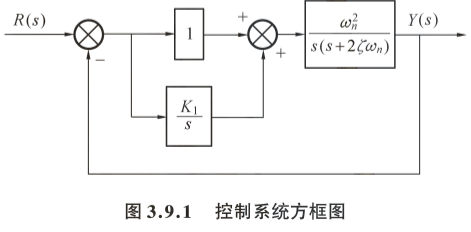
\includegraphics[width=.3\textwidth]{note/system stability/figure/1.png}
    \end{center}

    \textbf{解}： 图中闭环传递函数为：
    \begin{equation*}
        \varPhi(s) = \frac{Y(s)}{R(s)} = \frac{\omega_n^2(s+K_1)}{s^3 + 2\zeta\omega_n s^2 + \omega_n^2 s + K_1\omega_n^2}
    \end{equation*}

    由闭环传递函数求得系统的特征方程为：
    \begin{equation*}
        D(s) = s^3 +34.6 s^2 +7500 s +7500 K_1 = 0
    \end{equation*}

    列出相应的Routh行列表：
    \begin{equation*}
        \begin{array}{ccc}
            s^3 & 1 & 7500 \\
            s^2 & 34.6 & 7500 K_1 \\
            s^1 & \frac{34.6\times 7500 - 7500 K_1}{34.6} & 0 \\
            s^0 & 7500 K_1 & \\
        \end{array}
    \end{equation*}

    按照Routh行列表第一列各元全大于零的条件，应当满足下列不等式：
    \begin{equation*}
        \begin{split}
            \frac{34.6\times 7500 - 7500 K_1}{34.6} &>0 \\
            7500K_1 &>0
        \end{split}
    \end{equation*}

    故$0<K_1<34.6$
\end{example}

\subsection{确定某些参数间的相互关系}

\begin{example}
    单位负反馈系统的开环传递函数为：
    \begin{equation*}
        G(s) = \frac{K}{s(Ts+1)(2s+1)} \quad (K>0,T>0)
    \end{equation*}
    \begin{itemize}
        \item[(1)]为使闭环系统稳定，$K$和$T$应当满足什么关系？在$K-T$执教坐标系中画出使闭环系统稳定的区域。\\
        \textbf{解}：系统的特征方程为：
        \begin{equation*}
            D(s) = s(Ts+1)(2s+1) + K = 2Ts^3 +(2+T)s^2 +s +K =0
        \end{equation*}
        列出Routh行列表：
        \begin{equation*}
            \begin{array}{ccc}
                s^3 & 2T & 1 \\
                s^2 & 2+T & K \\
                s^1 & \frac{2+T-2KT}{2+T} & 0\\
                s^0 & K & \\
            \end{array}
        \end{equation*}

        由Routh行列表可知：$K< \dfrac{1}{T} + \dfrac{1}{2}$，画出$K-T$图如下：
        \begin{center}
            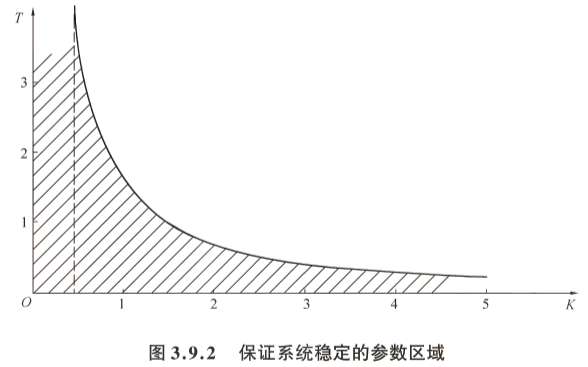
\includegraphics[width=.3\textwidth]{note/system stability/figure/2.png}
        \end{center}

        \item[(2)]若闭环系统处于临界稳定，持续振荡频率为1rad/s，求$K$和$T$的值\\
        \textbf{解}：若系统有频率为$\omega = 1$rad/s的持续振荡，说明系统的特征方程有一对纯虚根$\pm$j。根据特征方程出现纯虚根和Routh行列表的关系有：$K = \dfrac{1}{T}+\dfrac{1}{2}$。
        
        由$s^2$行得到辅助方程：
        \begin{equation*}
            (2+T)s^2 + K = 0
        \end{equation*}
        
        代入纯虚根可以解得：$T = \dfrac{1}{2},K=\dfrac{5}{2}$
    \end{itemize}
\end{example}

\subsection{保证系统稳定并且闭环极点远离虚轴}

\begin{example}
    系统方框图如下所示。要求闭环系统的特征根全在$s = -1 \pm j\omega$线左侧，试确定参数$K$的取值范围
    \begin{center}
        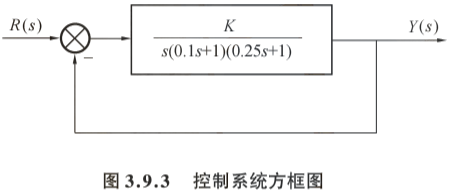
\includegraphics[width = .2\textwidth]{note/system stability/figure/3.png}
    \end{center}

    \textbf{解}：由方框图可以得到系统的特征方程为：
    \begin{equation*}
        s^3 + 14s^2 + 40s + 40K = 0
    \end{equation*}

    令$s = z - 1$，代入上式可得：
    \begin{equation*}
        z^3 + 11 z^2 + 15 z + (40K - 27) = 0
    \end{equation*}

    列出Routh行列表：
    \begin{equation*}
        \begin{array}{ccc}
            z^3 & 1 & 15 \\
            z^2 & 11 & 40K - 27 \\
            z^1 & \frac{11\times 155 - (40K-27)}{11} & 0 \\
            z^0 & 40K-27 & \\
        \end{array}
    \end{equation*}

    由Routh表可以得到以下不等式成立：
    \begin{equation*}
        \begin{split}
            11\times  15 -(40K-27) & >0 \\
            40K-27 &>0
        \end{split}
    \end{equation*}

    故$0.675<K<4.8$
\end{example}

\section{线性控制系统的稳态误差}

\subsection{控制系统的误差与稳态误差}

\begin{definition}{误差}
    在控制系统工作的时候，我们将期望的输出信号$y_r(t)$与实际的输出信号$y(t)$之差定义为\textbf{误差}，记为：
    \begin{equation*}
        e(t) \triangleq y_r(t)-y(t)
    \end{equation*}
\end{definition}

\begin{definition}{稳态误差}
    稳态误差的定义是误差信号的稳态值，记为：
    \begin{equation*}
        e_{ss} = \lim_{t\rightarrow \infty} e(t)
    \end{equation*}

    对于单位反馈系统，稳态误差可以由偏差信号的稳态值求得：
    \begin{equation*}
        e_{ss} = \lim_{t\rightarrow \infty} \varepsilon (t)
    \end{equation*}
\end{definition}

\subsection{终值定理和稳态误差的计算}

为了下面讨论问题方便，将单位反馈系统的开环传递函数写成典型环节形式：
\begin{equation*}
    G(s) = \frac{K\prod _{i=1}^m (\tau_i s + 1)}{s^v \prod_{j=1}^k (T_j s + 1) \prod _{k=1}^r (T_k^2 s^2 + 2\zeta_k T_k s + 1)}
\end{equation*}
其中$K$代表开环放大倍数，$v$代表开环传递函数中串联积分环节的个数

故此系统的稳态误差可以用Laplace变换的终值定理来求：
\begin{equation*}
    e_{ss} = \lim_{t\rightarrow \infty} e(t) = \lim_{s\rightarrow 0} s \varPhi_\varepsilon (s) R(s) = \lim_{s\rightarrow 0} s \frac{1}{1+G(s)} R(s) 
    = \lim_{s\rightarrow 0} s \frac{s^v \prod_{j=1}^q (\tau_j s + 1) \prod_{k=1}^r (T_k^2 s^2 + 2\zeta_k T_k s + 1)}{s^v \prod_{j=1}^q (T_j s + 1) \prod_{k=1}^r (T_k^2 s^2 + 2\zeta_k T_k s + 1) + K\prod_{i=1}^m (\tau_i s +1)} R(s)
\end{equation*}


由上式可以看出误差信号是与输入信号有关的，故下面将对不同的典型输入信号推导计算稳态误差：

\subsubsection{单位阶跃输入}

由上面可以知道：
\begin{equation*}
    e_{ss} = \lim_{t \rightarrow \infty}e(t) = \lim_{s\rightarrow 0} s E(s) = \lim_{s\rightarrow 0}s\frac{1}{1+G(s)}R(s) = \frac{1}{1+\lim_{s\rightarrow 0} G(s)}
\end{equation*}

观察到$e_{ss}$只与$\lim_{s\rightarrow 0} G(s)$有关，故定义静态位置误差系数：
$K_p = \lim_{s\to 0} G(s) = \begin{cases}
K&\quad v=0 \\
\infty &\quad v\geq 1
\end{cases}$


由上述定义可知单位阶跃作用下稳态误差的计算公式：
\begin{equation*}
    e_{ss} = \begin{cases}
        \frac{1}{1+K_p} &\quad v=0\\
        0 & \quad v\geq 1
    \end{cases}
\end{equation*}

\begin{definition}{系统的分类}
    开环传递函数终，串联积分环节数$v$对于控制系统的稳态误差起着重要的作用，为了区别各自特点，将系统根据$v$的值进行分类：
    \begin{enumerate}
        \item $v=0$：0型系统
        \item $v=1$：I型系统
        \item $v=2$：II型系统
        
        $\vdots$

        对于III型及以上的系统，使系统稳定是十分困难的，所以除非由特殊需要，一般很少采用III型及以上的控制系统
    \end{enumerate}
\end{definition}

\subsubsection{单位斜坡输入}

由上面可知稳态误差可以用下式计算：
\begin{equation*}
    e_{ss} = \lim_{s\to 0}s\frac{1}{1+G(s)} \frac{1}{s^2} = \lim_{s\to 0}\frac{1}{sG(s)}
\end{equation*}

定义$K_v$为系统的静态速度误差系数
\begin{equation*}
    K_v = \lim_{s\to 0} sG(s) = \begin{cases}
        0 & \quad v=0\\
        K & \quad v=1\\
        \infty & \quad v=2\\
    \end{cases}
\end{equation*}

代入上式可得：
\begin{equation*}
    e_{ss} = \begin{cases}
        \infty & \quad v=0\\
        \frac{1}{K_v} & \quad v=1\\
        0 & \quad v=2 \\
    \end{cases}
\end{equation*}

\subsubsection{单位加速度输入}
由上面可知稳态误差可以用下式计算：
\begin{equation*}
    e_{ss} = \lim_{s\to 0}s \frac{1}{1+G(s)} \frac{1}{s^3} = \lim_{s\to 0}\frac{1}{s^2 G(s)}
\end{equation*}

定义$K_a$为系统的静态加速度误差系
\begin{equation*}
    K_a = \lim_{s\to 0}s^2G(s) = \begin{cases}
        0 & \quad v=0\\
        0 & \quad v=1 \\
        K & \quad v=2\\
    \end{cases}
\end{equation*}

代入上式可得：
\begin{equation*}
    e_{ss} = \begin{cases}
        \infty & \quad v=0\\
        \infty & \quad v=1 \\
        \frac{1}{K_a} & \quad v=2\\
    \end{cases}
\end{equation*}

用一个表把上述三个信号作用下的稳态误差总结为：
\begin{center}
    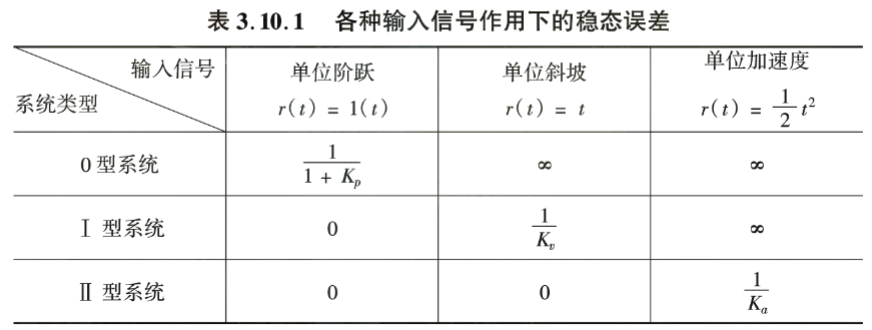
\includegraphics[width = .6\textwidth]{note/system stability/figure/4.png}
\end{center}

\subsection{干扰信号作用下的稳态误差}

主要思路：求出在$R(s) = 0$时由干扰信号引起的偏差函数$E_f(s) = \varPhi_{ef}(s)F(s)$，最后用终值定理即可求出由误差信号引起的偏差信号（单位反馈系统满足叠加定理）

\subsection{动态误差系数}

偏差信号的Laplace变换式为：
\begin{equation*}
    E(s) = \varPhi_e(s) R(s)
\end{equation*}

将偏差的闭环传递函数在$s=0$的邻域内展开成Taylor级数：
\begin{equation*}
    \varPhi_e(s) = \frac{1}{i!}\Sigma_{i=0}^\infty \varPhi_e^{(i)}(0) s^i
\end{equation*}

称$\dfrac{1}{i!}\varPhi_e^{(i)}(0)\quad (i\in Z)$为系统的动态误差系数

代入偏差信号的Laplace变换式后对其做Laplace反变换有：
\begin{equation*} 
    e_{ss}(t) = \frac{1}{i!}\Sigma_{i=0}^\infty \varPhi_e^{(i)}(0)r^{(i)}(t)
\end{equation*}

一种求动态误差系数的方法：一般$\varPhi_e(s)$为有理分式形式，对有理分式做大除法即可得到$\varPhi_e(s)$按s的升幂级数排列形式

\section{根轨迹法}

\subsection{基本概念}

考虑如图所示的闭环控制系统，其闭环传递函数为：
\begin{center}
    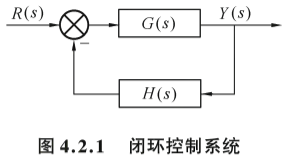
\includegraphics[width=.2\textwidth]{note/system stability/figure/5.png}
\end{center}
\begin{equation*}
    \varPhi(s) = \frac{Y(s)}{R(s)} = \frac{G(s)}{1+G(s)H(s)}
\end{equation*}

系统的特征方程为：$1+G(s)H(s) = 0$，将系统的开环传递函数写成如下零极点形式：
\begin{equation*}
    G(s)H(s) = \frac{k\prod_{i=1}^m (s-z_i)}{\prod_{j=1}^n (s-p_j)}
\end{equation*}

其中，$z_1,z_2,\cdots,z_m$和$p_1,p_2,\cdots,p_n$分别为系统的开环零点和极点，根据上述特征方程我们可以得到以下两个结论：
\begin{equation*}
    \begin{split}
        \left\lvert G(s)H(s) \right\rvert &= \frac{k\prod_{i=1}^m \left\lvert s-z_i \right\rvert }{\prod_{j=1}^n \left\lvert s-p_j \right\rvert } = 1 \\
        \angle G(s)H(s) &= \Sigma_{i=1}^m \angle(s-z_i) - \Sigma_{j=1}^n \angle(s-p_i) = \pm(2l+1)\pi \quad (l\in N)
    \end{split}
\end{equation*}

上述两式称为根轨迹方程，第一条称为根轨迹的幅值条件，第二条称为根轨迹的幅角条件

\begin{ascolorbox9}{画根轨迹的主要步骤}
    \begin{enumerate}
        \item 把系统的开环传递函数写成零极点形式
        \item 在$s$平面上画出开环零点和极点，一般用“$ \odot $”表示开环零点，用“$\times$”表示开环极点
        \item 在$s$平面上找出满足幅角条件的点，这些点连接成根轨迹。
        \item 对于根轨迹上的一些必要的点，利用幅值条件式求出他们所对应的$k$值，还可以进一步求出对应的开环放大倍数$K$
    \end{enumerate}
\end{ascolorbox9}

\subsection{绘制根轨迹的基本规则}

由上可知：负反馈闭环控制系统的特征方程为：
\begin{equation*}
    G(s) H(s) = -1
\end{equation*}

根轨迹的幅角条件为：
\begin{equation*}
    \angle G(s) H(s) = \Sigma_{i=1}^m \angle(s-z_i) - \Sigma_{j=1}^n \angle(s-p_j) = (2l+1)\pi
\end{equation*}

当根轨迹增益$k$由$0\to \infty$时，按照上述条件绘制的根轨迹称做负反馈根轨迹，或称根轨迹。利用下面的一些规则，可以在$s$平面上找到满足上述条件的点，从而绘制出根轨迹：
\begin{ascolorbox4}{根轨迹绘制八大法则}
    \begin{enumerate}
        \item \textbf{根轨迹的起点与终点}：根轨迹起始于开环极点，终止于开环零点；如果开环极点个数n大于开环零点个数m，则有n-m条根轨迹终止于无穷远处（无穷远点属于开环零点）
        \item \textbf{根轨迹的分支数，对称性和连续性}：根轨迹的分支数=开环极点数；根轨迹连续且对称于实轴
        \item \textbf{实轴上的根轨迹}：从实轴上最右端的开环零、极点算起，奇数开环零、极点到偶数开环零、极点之间的区域必是根轨迹（不区分该点是零点还是极点）

        以下图作为例子，红线部分为根轨迹：
        \begin{center}
            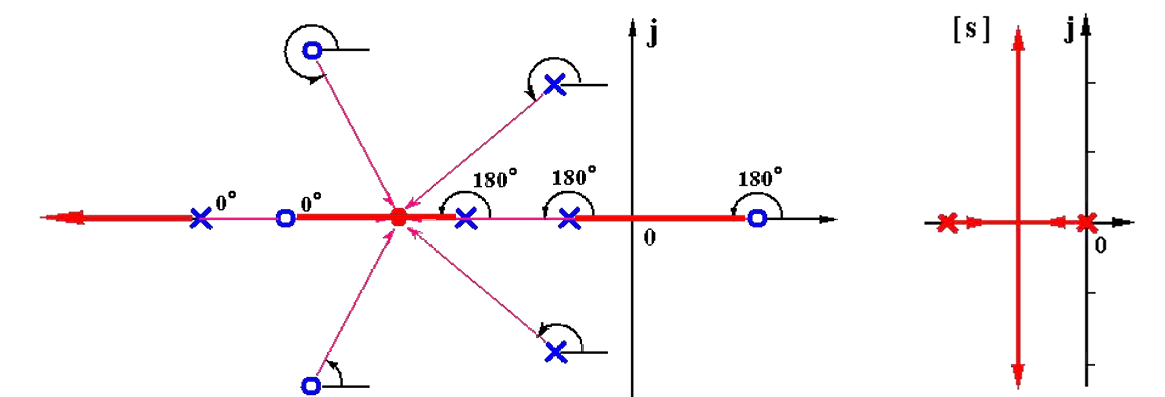
\includegraphics[width=.6\textwidth]{note/system stability/figure/6.png}
        \end{center}
        \item \textbf{闭环特征方程根之和}：当开环极点个数n与开环零点个数m之差大于2（n-m>2）时， 闭环特征方程根的和保持为一个常值，亦可写为：一部分根左移，另一部分根必然右移，且移动总量为0
        \item \textbf{根轨迹的渐近线}：当开环极点个数大于开环零点个数时，根轨迹的渐近线必定存在，且可用以下式子表示：
        \begin{equation*}
            \begin{split}
                \text{实轴截距：}& \sigma_a = \frac{\Sigma_{i=1}^n p_i - \Sigma_{j=1}^m z_j}{n-m} \\
                \text{倾斜角：}& \varphi_a = \frac{(2k+1)\pi}{n-m} \quad (k\in Z)
            \end{split}
        \end{equation*}
        \item \textbf{分离点求法}：设分离点为$d$（重根值），则分离点可由以下式子给出：
        \begin{equation*}
            \Sigma_{i=1}^n \frac{1}{d-p_i} = \Sigma_{j=1}^m \frac{1}{d-z_j}
        \end{equation*}
        \begin{equation*}
            \text{或}\frac{dD(s)}{ds} = 0 \text{的根}
        \end{equation*}
        \item \textbf{与虚轴交点的求法}：根轨迹与虚轴交点满足以下两个性质：
        \begin{itemize}
            \item[(I)] 该点时系统的临界稳定点
            \item[(II)] $s=j\omega \quad (\omega\in \mathbb{R})$ 
        \end{itemize}
        
        将上述两个性质任意一条代入闭环特征方程中即可求得根轨迹与虚轴交点
        \item \textbf{出射角/入射角（起始角/终止角）}：用幅角方程$\Sigma_{i=1}^m \angle(s-z_i) - \Sigma_{j=1}^n \angle(s-p_i) = \pm(2l+1)\pi$即可求得在起始点的幅角和终值点的幅角
        \item 定理（一种特殊情况）：若系统有2个开环极点，1个开环零点，且在复平面存在根轨迹，则复平面的根轨迹一定是以该零点为圆心的圆弧
    \end{enumerate}
\end{ascolorbox4}

\subsection{根轨迹法分析控制系统性能}
\begin{example}
    负反馈系统的开环传递函数为：
    \begin{equation*}
        G(s)H(s) = \frac{k(s+1)}{s(s-3)}
    \end{equation*}

    试用根轨迹分析该系统的性能

    \textbf{解}：给出的系统开环传递函数已是典型的零、极点形式，可以直接求出开环极点是$p_1 = 0,p_2 = 3,n=2$；开环零点是$z_1 = -1,m=1$

    同时可以求出分离点$d_1 = 1,d_2 = -3$；与虚轴交点$\pm j \sqrt{3}$，渐近线为实轴，画出根轨迹图如下：
    \begin{center}
        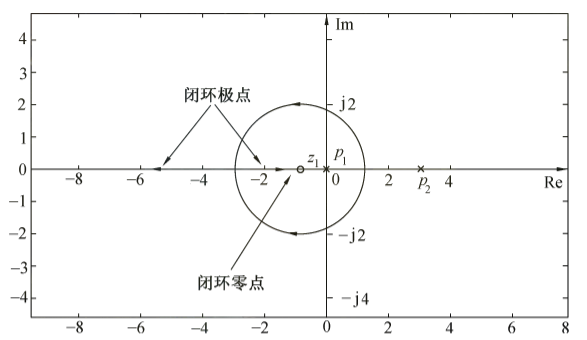
\includegraphics[width=.3\textwidth]{note/system stability/figure/7.png}
    \end{center}

    \begin{itemize}
        \item[(1)] 分析稳定性：该闭环负反馈系统，在开环放大倍数$K<1$时系统不稳定
        \item[(2)] 动态过程分析：根轨迹实轴上-3处回合分离点对应的$k=9$，开环放大倍数$K=3$。当$1<K<3$时，闭环传递函数有一对共轭的复数极点和一闭环极点$z_1 = -1$，系统是稳定的，但动态过程中会出现衰减振荡的分量；当$k>9,K>3$时，系统的闭环传递函数有两个负实数极点和一个零点$z_1=-1$，系统稳定，动态过程中无衰减振荡分量。由于系统的闭环传递函数中存在一个零点$z_1 = -1$和两个极点，所以需要用Laplace反变换或用MATLAB求取系统的阶跃响应曲线，再求出各项动态性能指标
        \item[(3)] 稳态误差分析：该系统的开环传递函数有一个$p_1 = 0$的极点，所以系统是I型系统。根据闭环极点的位置可以求出该店对应的$k$与$K$的值，开环放大倍数$K = K_v$，可以由此计算出稳态误差
    \end{itemize}
\end{example}

\subsection{特殊根轨迹}

\subsubsection{正反馈系统的根轨迹}
正反馈系统的特征方程为：
\begin{equation*}
    1-G(s)H(s) = 0
\end{equation*}

转化为幅值条件和相角条件为：
\begin{equation*}
    \begin{split}
        \left\lvert G(s)H(s)\right\rvert  &= \frac{k\prod_{i=1}^m\left\lvert (s-z_i)\right\rvert }{\prod_{j=1}^n \left\lvert (s-p_j) \right\rvert } = 1\\
        \angle G(s)H(s) &= \Sigma_{i=1}^m\angle(s-z_i) - \Sigma_{j=1}^n \angle(s-p_j) = 2l\pi
    \end{split}
\end{equation*}

因此，上述八大法则存在一定的偏差，不同之处为：
\begin{enumerate}
    \item 法则3：实轴上的根轨迹：从实轴上最右端的开环零、极点算起，偶数开环零、极点到奇数开环零、极点之间的区域必是根轨迹（不区分该点是零点还是极点）
    \item 法则5：渐近线的倾斜角：$\varphi_a = \dfrac{2l\pi}{n-m}$
    \item 法则8：入射角/出射角计算：$\Sigma_{i=1}^m\angle(s-z_i) - \Sigma_{j=1}^n \angle(s-p_j) = 2l\pi$
\end{enumerate}

\subsubsection{参数根轨迹}

绘制反馈系统的根轨迹时，其参变量并不一定是系统的开环增益。为了区别以开环增益为参变量的一般根轨迹，把以非开环增益的其他参数作为参变量的根轨迹称作\textbf{反馈系统的参数根轨迹}

计算此种形式的一般方法：构造“等效开环传递函数”，将参数根轨迹化为一般根轨迹
\begin{example}
    已知负反馈系统的开环传递函数为：
    \begin{equation*}
        G(s)H(s) = \frac{2}{s(\tau s + 1){s+1}}
    \end{equation*}

    试绘制以参数$\tau$为参变量的参数根轨迹。

    \textbf{解}：原系统的特征方程为：
    \begin{equation*}
        D(s) = s(\tau s +1)(s+1) + 2 = \tau s^2 (s+1) + s(s+1) + 2 = 0
    \end{equation*}

    构造开环传递函数：
    \begin{equation*}
        \overline{G}(s) \overline{H}(s) = \frac{\tau s^2 (s+1)}{s (s+1) + 2}
    \end{equation*}

    根据八大规则可以绘制根轨迹如下：
    \begin{center}
        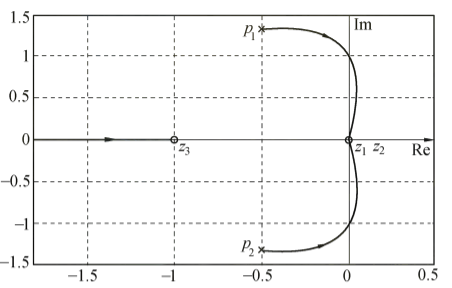
\includegraphics[width = .3\textwidth]{note/system stability/figure/8.png}
    \end{center}
\end{example}

\section{Nyquist稳定性判据}
在介绍Nyquist稳定判据前，我们先了解一个引理：
\begin{lemma}{对数留数定理}
    设$f(z)$在简单闭曲线$C$上处处解析且不等于0，在$C$内除去有限个极点$b_j(1\leq j \leq m)$外也处处解析，且在$C$内有零点$a_k(1\leq k \leq n)$，$\varphi(z)$在$C$上及内部均解析，则：
    \begin{equation*}
        \frac{1}{2\pi i}\oint_C \varphi(z) \frac{f'(z)}{f(z)}dz = \sum_{k=1}^n \alpha_k \varphi(a_k) -\sum_{j=1}^m \beta_j \varphi(b_j)
    \end{equation*}

    其中$\alpha_k$为$a_k$的阶数，$\beta_j$为$b_j$的阶数，$C$取正方向

    特别地，若$\varphi(z)\equiv 1$，有：
    \begin{equation*}
        \frac{1}{2\pi i} \oint_C \frac{f'(z)}{f(z)}dz = \sum_{k=1}^n \alpha_k  -\sum_{j=1}^m \beta_j = Z - P
    \end{equation*}

    其中，$Z$为$f(z)$在$C$内的零点总个数，$P$为$f(z)$在$C$内的极点总个数（均计算重数）

    上式中$\dfrac{1}{2\pi i}\displaystyle{\oint_C \frac{f'(z)}{f(z)}}$称为对数留数，其几何意义为：当点$z$沿$C$的正方向绕行一周后幅角$\Delta_C \arg f(z)$的改变量的$\dfrac{1}{2\pi}$倍，或$w = f(z)$在$w$平面内沿闭曲线$\Gamma_w$绕原点的圈数
\end{lemma}

此时我们就可以引出Nyquist稳定判据的定义：
\begin{definition}
    对于一个LTI系统，设$Z$为在右半平面中的闭环极点个数，$P$为在右半平面中的开环极点个数，$N$为s沿开环Nyquist曲线穿过$(-1,j0)$点左侧负实轴的次数，则有：
    \begin{equation*}
        Z = P - 2N
    \end{equation*}

    显然，当$Z=0$时系统是稳定的，$Z>0$时系统是不稳定的

    当开环系统中含有积分环节时，对应的Nyquist曲线需要从$\omega = 0$到$\omega=0^+$顺时针补充半径为$\infty$，角度为$v\times \dfrac{\pi}{2}$的圆弧
\end{definition}

注意到在上述定义中有涉及“穿越”，下面给出“穿越”的定义：
\begin{definition}
    对于Nyquist曲线，我们认为其从第二象限穿越$(-1,j0)$左侧负实轴至第四象限为正穿越，反之为负穿越

    半次穿越：Nyquist曲线起始或终止于$(-1,j0)$左侧负实轴，此时记穿越为半次穿越，正负值定义同上

    穿越的示意图如下所示：
    \begin{center}
        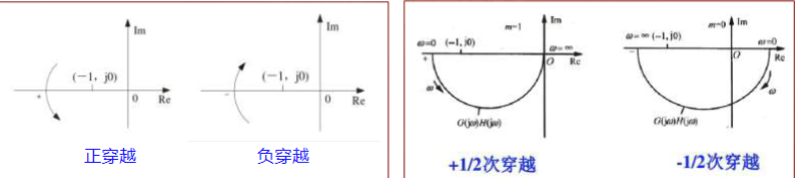
\includegraphics[width = .5\textwidth]{note/system stability/figure/9.png}
    \end{center}
\end{definition}

\begin{example}
    （此例题摘自上课ppt）
    \begin{center}
        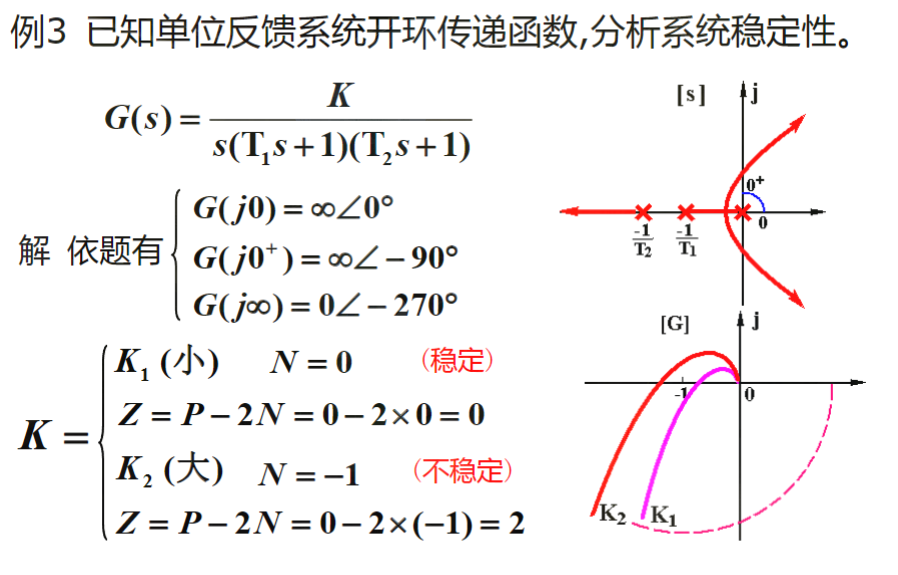
\includegraphics[width = .5\textwidth]{note/system stability/figure/10.png}
    \end{center}
\end{example}

\section{线性离散系统的稳定性}

\subsection{$s$平面到$z$平面的映射关系}

在定义Z变换时，我们定义了复变量$s$与复变量$z$之间的转换关系为：
\begin{equation*}
    z = e^{Ts}
\end{equation*}
将$s = \sigma + j \omega $带入可以得到：
\begin{equation*}
    z = e^{(\sigma + j \omega)T} = e^{\sigma T} e^{j\omega T} = \left\lvert z \right\rvert e^{j\omega T}
\end{equation*}
于是我们可以得到$s$平面到$z$平面的基本映射关系为：
\begin{equation*}
    \left\lvert z \right\rvert = e^{\sigma T} \quad \angle z = \omega T
\end{equation*}
观察上式可以得到：$s$平面的虚轴在$z$平面的映像为单位圆，$s$左半平面在$z$平面的映像为单位圆内，$s$右半平面在$z$平面的映像为单位圆外，具体如下图所示：
\begin{center}
    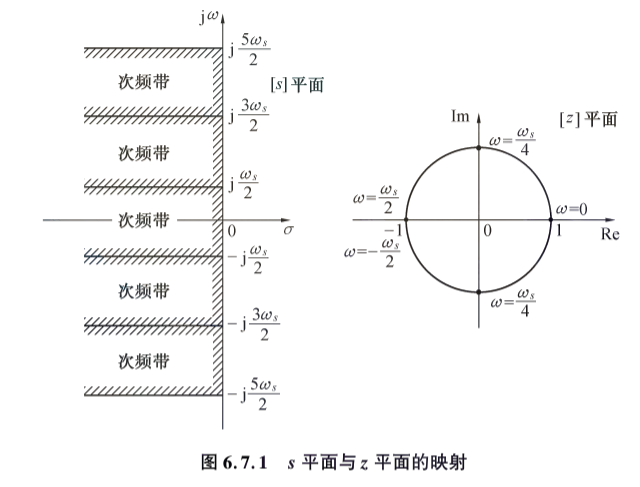
\includegraphics[width = .5\textwidth]{note/system stability/figure/11.png}
\end{center}

\subsection{线性离散系统稳定的充要条件}

首先，我们先假设闭环线性离散系统的特征方程的根，或闭环脉冲传递函数的极点为$z_1,z_2,\cdots,z_n$，则线性离散系统稳定性具有如下定理：
\begin{theorem}
    线性离散系统稳定的充要条件为：线性离散系统的全部特征根$z_i\, (i=1,2,\cdots,n)$都分布在$z$平面的单位圆内，或者说全部特征根的模都必须小于1，即：$\left\lvert z_i \right\rvert <1 \,(i=1,2,\cdots,n) $。如果在上述特征根中，有位于$z$平面单位圆之外者时，闭环系统将是不稳定的
\end{theorem}

\subsection{Routh稳定判据}

在线性离散系统中，判断稳定性需要判别特征方程的根是否在$z$平面的单位圆内，但是在连续系统中，Routh判据是判断极点是否在左半平面。故在线性离散系统中，不能直接使用Routh判据。为了使用Routh判据，需要将稳定区域映射到新平面的左半平面，故此时引入$w$变换，将$z$平面上单位圆内部区域，映射到$w$平面的左半平面，即：
\begin{equation*}
    w = \frac{z+1}{z-1}
\end{equation*}

两个平面间的映射关系由下图表示：
\begin{center}
    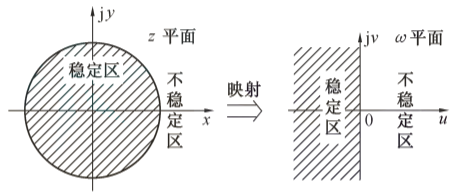
\includegraphics[width = .6\textwidth]{note/system stability/figure/12.png}
\end{center}

显然，$w$变换是线性变换的一种，且其可逆。$z$的有理多项式经过$w$变换之后，可以得到$w$的有理多项式。以$z$为变量的特征方程经过$w$变换之后得到以$w$为变量的特征方程，就可以应用Routh判据来判断线性离散系统的稳定性

\begin{example}[摘自课本例题6.7.3]
    \begin{center}
        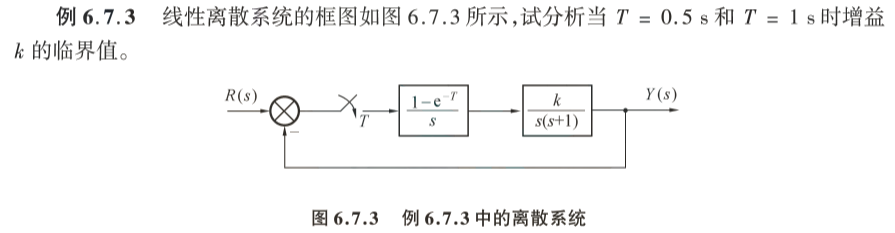
\includegraphics[width = .8\textwidth]{note/system stability/figure/13.png}\\
        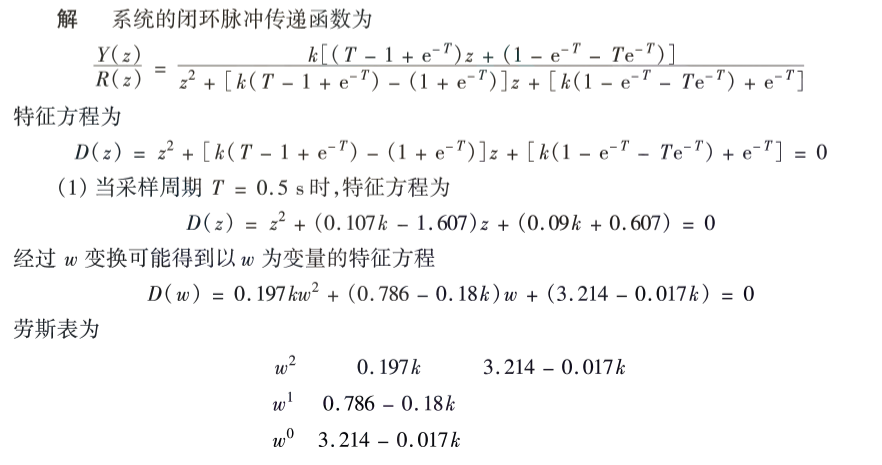
\includegraphics[width = .8\textwidth]{note/system stability/figure/14.png}\\
        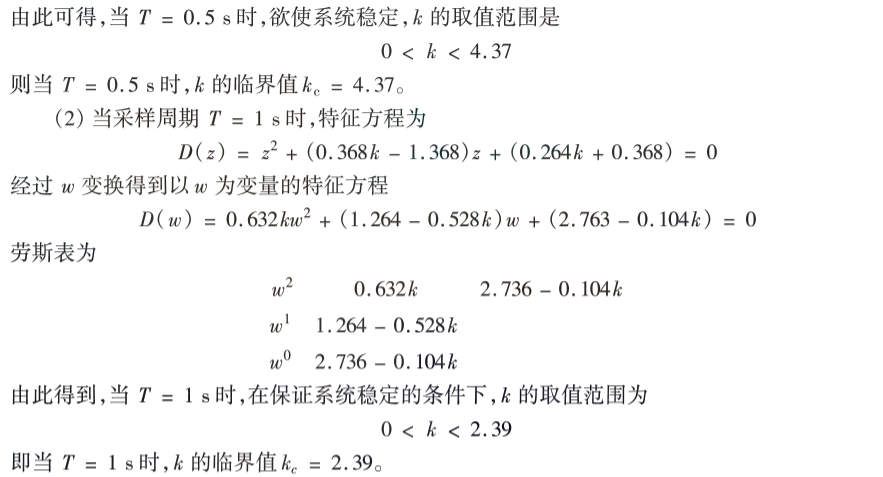
\includegraphics[width = .8\textwidth]{note/system stability/figure/15.png}
    \end{center}
\end{example}

\subsection{线性离散系统的稳态误差}

\subsubsection{稳态误差与稳态误差终值}

和连续系统类似，离散系统的误差信号的脉冲序列$e^* (t)$反映了在采样时刻系统希望输出与实际输出之差，当$t \geq t_s$，即过渡过程结束后，系统误差信号的脉冲序列就是离散系统的稳态误差。一般记为
\begin{equation*}
    e^*_{ss}(t) \quad t\geq t_s
\end{equation*}
同样的，当$t \to \infty$时，可以求得线性离散系统在采样点上的稳态误差终值：
\begin{equation*}
    e^*_{ss}(\infty) = \lim_{t\to \infty} e^* (t) = \lim _{t \to \infty} e^*_{ss}(t)
\end{equation*}
如果误差信号的Z变换为$E(z)$，在满足Z变换终值定理使用条件的情况下，可以利用Z变换的中值定理求离散系统稳态误差的终值
\begin{equation*}
    e^*_{ss}(\infty) = \lim_{t\to \infty} e^* (t) = \lim_{z\to 1}(z-1)E(z)
\end{equation*}

\subsubsection{稳态误差系数}
和连续系统类似，线性离散系统也存在几个静态误差系数，具体为：
\begin{enumerate}
    \item 静态位置误差系数：$K_p = \lim\limits_{z\to 1} GH(z)$
    \item 静态速度误差系数：$K_v = \lim\limits_{z\to 1} (z-1)GH(z)$
    \item 静态加速度误差系数：$K_a = \lim\limits_{z\to 1} (z-1)^2 GH(z)$
\end{enumerate}

\begin{center}
    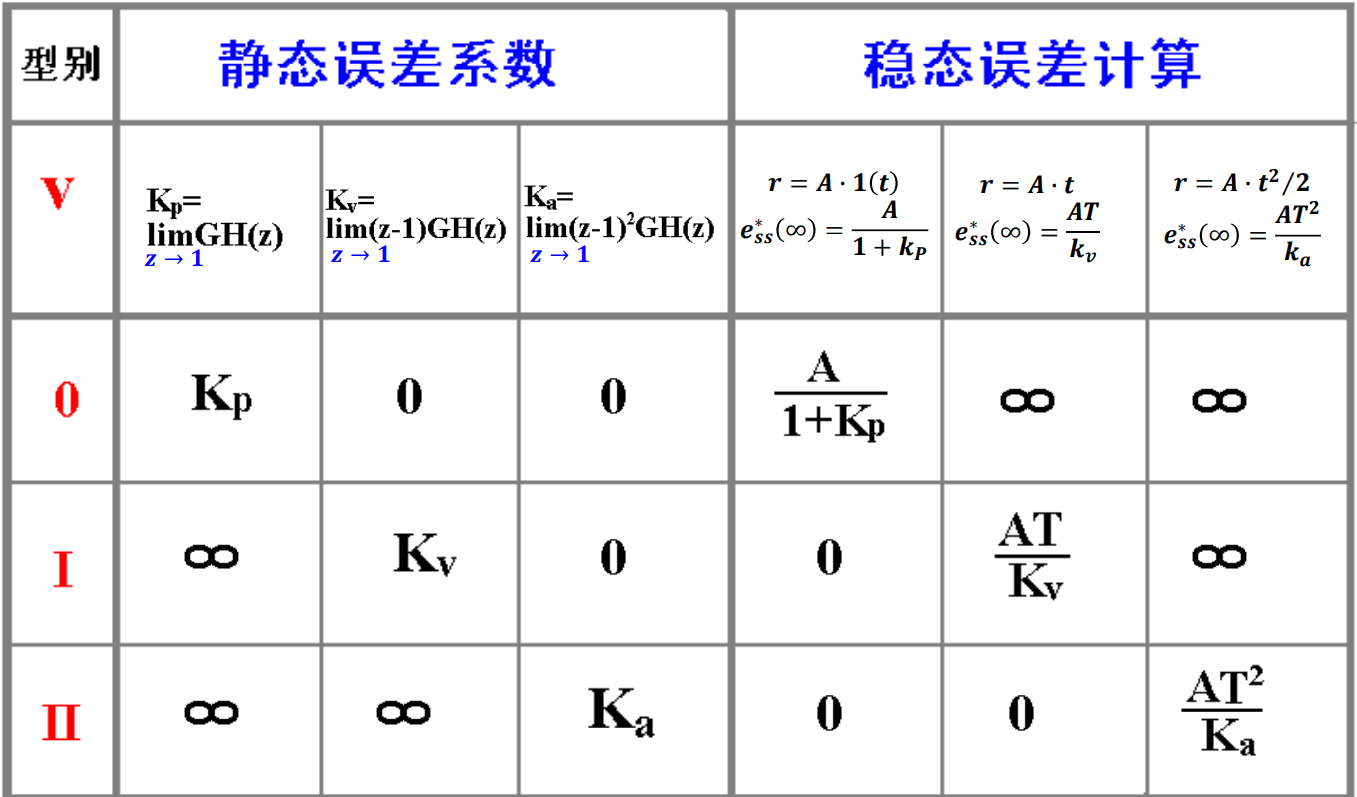
\includegraphics[width = .6\textwidth]{note/system stability/figure/16.png}
\end{center}

\subsubsection{动态误差系数}

与连续系统类似，我们也可以定义离散系统的动态误差系数

若系统闭环误差传递函数为$\Phi_e(z)$，根据Z变换的定义，将$z = e^{sT}$代入$\Phi_e(z)$，可以得到以$s$为变量的闭环误差脉冲传递函数：
\begin{equation*}
    \Phi_e^* (s) = \Phi_e^* (z) \left|_{z = e^{sT}}  \right.
\end{equation*}

\begin{center}
    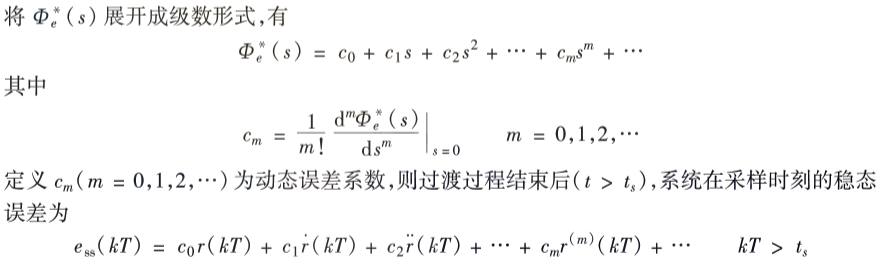
\includegraphics[width = .9\textwidth]{note/system stability/figure/17.png}
\end{center}